\documentclass[12pt,letterpaper]{article}

\usepackage{amsmath} % do komendy \text
\usepackage[margin=0.8in]{geometry}
\usepackage[english]{babel}
\usepackage[utf8]{inputenc}
\usepackage{hyperref}
\usepackage{indentfirst}
\usepackage{graphicx}
\usepackage{fontenc}
\usepackage{caption}
\usepackage{subcaption}
\usepackage{array}
\usepackage{cleveref}
\usepackage{float}
\usepackage{mhchem}
\usepackage{multirow}
\usepackage{stackengine}
\usepackage[backend=biber,style=numeric, sorting=none]{biblatex}

%for showing python code:
\usepackage{listings}
\usepackage{xcolor}
\lstset{
    language=Python, % Set programming language
    basicstyle=\ttfamily\small, % Style of the code font
    keywordstyle=\color{blue}, % Color for keywords
    stringstyle=\color{green!60!black}, % Color for strings
    commentstyle=\color{red}, % Color for comments
    numbers=left, % Line numbers (can be none, left, or right)
    numberstyle=\tiny\color{gray}, % Style for line numbers
    stepnumber=1, % Step between two line numbers
    frame=single, % Adds a frame around the code
    tabsize=4, % Sets tab space
    breaklines=true, % Automatic line breaking
    breakatwhitespace=true, % Break only at whitespace
    showstringspaces=false, % Don't display spaces in strings
    backgroundcolor=\color{lightgray}, % Set background color
    frame=single, % Add a frame around the code
    rulecolor=\color{black} % Set frame color
}

\addbibresource{references.bib} 

\newlength{\bibparskip}\setlength{\bibparskip}{0pt}
\let\oldthebibliography\thebibliography
\renewcommand\thebibliography[1]{%
  \oldthebibliography{#1}%
  \setlength{\parskip}{\bibitemsep}%
  \setlength{\itemsep}{\bibparskip}%
}
\newcolumntype{M}[1]{>{\centering\arraybackslash}m{#1}}
\newcolumntype{P}[1]{>{\centering\arraybackslash}p{#1}}
\newcommand\xrowht[2][0]{\addstackgap[.5\dimexpr#2\relax]{\vphantom{#1}}}

%my commands
\newcommand{\txt}[1]{\textit{#1}}
\newcommand{\degreeCelsius}{$^\circ$C}
\newcommand{\degree}{$^\circ$}
\newcommand{\nid}{\noindent}
\newcommand{\angstrom}{\mbox{\normalfont\AA}}%do pisania angstremów
\newcommand{\Frac}[2]{\left(\frac{#1}{#2}\right)}
\setlength{\parindent}{3em}

\begin{document}

\begin{center}
    \begin{huge}
     Information distillation from physical simulation\\[12pt]
    \end{huge}
    Damian Gierek\\
    \vspace{0.1em}
    07.02.2025
\end{center}

\hspace{0.3em}

\nid In this paper, I use the method of unsupervised learning of equations of motion for objects in unlabelled synthetic video, presented in~\cite{Udrescu2021}, for the case of videos of bodies moving in gravitational field to obtain the trajectories of the bodies. To obtain this, I trained an autoencoder that maps each video frame into a low-dimensional latent space that allows reproducing the original image. The desired 2D Cartesian trajectory is obtained via principal component analysis of vectors from the latent space. The paper presents preliminary results.

\section{Motivation and methodology}

By obtaining the trajectory of a moving body from a video, we can guess the formula that governs the movement of the body using symbolic regression. An example of an algorithm that allows it is "AI Feynman" \cite{udrescu2020}. This approach was analogous to the work of Johannes Kepler, who discovered that Mars' orbit is an ellipse after analysing the data of its orbit \cite{koyre2013}. 

The method is based on training a specific architecture consisting of an autoencoder and an evolution operator performed on a set of snapshots of a simulation of a body moving in a gravity field. In a sense we reproduce the approach of Kepler, however the hand work of the correct coordinate choice is done automatically by the neural network.

\section{Code library}
The whole code I used for the project is publicly available here: \url{https://github.com/dgierek/physics_guesser}. 

The library contains the module "data\_generator.py" that is responsible for generating simulation data. Module called "rocket\_simulation.py" stores the analytical solutions used in simulation generation. Simulations are stored in the file "simulation\_frames".

The module called "autoencoder.py" contains an implementation of used neural network architecture. Whilst "datasets.py" contains data loaders that inherit from torch.utilis.da-\\ta.Dataset and load the simulation data during training sessions. The training loop is implemented in "trainer.py".

Finally, in the "evaluator.py" module I implemented the method for calculating the loss function. The "evaluation.py" module stores the code that allows to visualize the model predictions of images.

\subsection{Simulation of a body moving in a gravity field}

The first problem to solve for the project was to create a training dataset for the neural network. In the beginning, I decided to simulate the movement in a gravitational, magnetic, harmonic field and the movement of a free point particle using numerical integration of differential equations of motion via the Verlet method. Then, I realised it is not necessary as using the analytical solutions is sufficient. Below I show the equations of motion for each type, the analytical solutions I used for simulation and an example of a generated trajectory:

\begin{itemize}
    \item gravity:
    \begin{flushleft}
        \begin{align*}
            \vec{F_g} & = m\vec{g}\\
            x(t) & = \frac{g_x\cdot t^2}{2} + V_{0,x} t + x_0\\
            y(t) & = \frac{g_y\cdot t^2}{2} + V_{0,y} t + y_0,
        \end{align*}
    \end{flushleft}
    \nid where $\vec{F_g}$ is the force of gravity, $m$ is mass of the body (in every calculation $m=1$ was assumed), $\vec{g}$ is the gravity acceleration vector and its $x$ and $y$ components: $g_x$, $g_y$, while $x(t)$, $y(t)$ is the $x$ and $y$ component of the position of the body at a given time $t$. $x_0$ and $y_0$ describe the initial position. $V_{0,x}$ and $V_{0,y}$ describe the initial velocity. An example trajectory was shown on the figure~\ref{fig:exmp_traj_grav}.

    \item magnetic field:
    \begin{flushleft}
        \begin{align*}
            m \ddot{x} & = q \cdot \dot{y} \cdot B_z\\
            m \ddot{y} & = -q \cdot \dot{x} \cdot B_z\\
            x(t) & = x_0 + \frac{1}{\omega}(v_{0,x} \sin{(\omega t)} + v_{0,y} (1 - \cos{(\omega t)}))\\
            y(t) & = y_0 + \frac{1}{\omega}(v_{0,x} (\cos{(\omega t)} - 1) + v_{0,y} \sin{(\omega t)}),
        \end{align*}
    \end{flushleft}
    \nid where double dots represent the second time derivative and single dot represent the first time derivative. $q$ is the electric charge of a body, $B_z$ is the $z$ component of the magnetic field vector (in the 2D case only this component influences the movement) and $\omega=\frac{qB_z}{m}$. An example trajectory was shown on the figure~\ref{fig:exmp_traj_magn}.

    \item harmonic oscillator:
    \begin{flushleft}
        \begin{align*}
            m \ddot{x} & = - k_x (x-r_{0,x})\\
            m \ddot{y} & = - k_y (x-r_{0,y})\\
            x(t) & = (x_0 - r_{0,x}) \cos({\omega_x t}) + \frac{v_{0,x}}{\omega_x} \sin{(\omega_x t)} + r_{0,x}\\
            y(t) & = (y_0 - r_{0,y}) \cos{(\omega_y t)} + \frac{v_{0,y}}{\omega_y} \sin{(\omega_y t)} + r_{0,y},
        \end{align*}
    \end{flushleft}
    \nid where $k_x$, $k_y$ are spring constants in directions $x$ and $y$, $r_{0,x}$ and $r_{0,y}$ are the coordinates of the equilibrium position of the harmonic oscillator (at this point the force acting on the body is $\vec{0}$). $\omega_x=\sqrt{\frac{k_x}{m}}$ and $\omega_y=\sqrt{\frac{k_y}{m}}$. An example trajectory called Lissajous curve was shown on the figure~\ref{fig:exmp_traj_harm}.

    \item free body movement:
     \begin{flushleft}
        \begin{align*}
            \vec{F_f} & = \vec{0}\\
            x(t) & = x_0 + v_{0,x}t\\
            y(t) & = y_0 + v_{0,y}t.
        \end{align*}
    \end{flushleft}
    \nid An example trajectory was shown on the figure~\ref{fig:exmp_traj_free}.

\begin{figure}[H]
    \centering

        \begin{minipage}{0.49\textwidth}
        
        \centering
        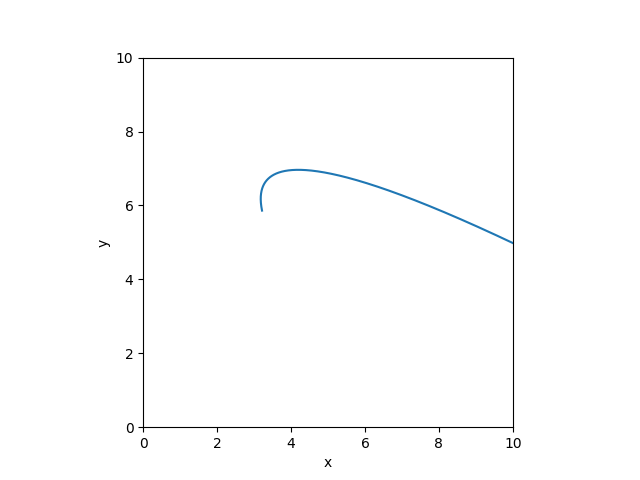
\includegraphics[width=1\linewidth]{example_trajectory_gravity.png}
        \caption{Example trajectory of a body moving in a gravity field. Parameters: $x_{0} = \text{3,22}$, $y_{0} =~\text{5,86}$, $V_{0,x} = -\text{0,17}$, $V_{0,y} = \text{0,82}$, $g_{x} = \text{0,40}$, $g_{y} = -\text{0,31}$.}
        \label{fig:exmp_traj_grav}
        
        \end{minipage}
    \hfill
        \begin{minipage}{0.49\textwidth}
        
        \centering
        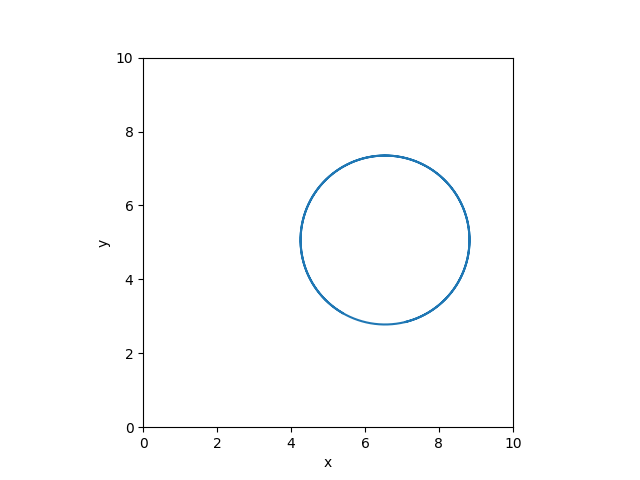
\includegraphics[width=1\linewidth]{example_trajectory_magnetic_field.png}
        \caption{Example trajectory of a body moving in a magnetic field. Parameters: $x_{0} = \text{5,40}$, $y_{0} =~\text{3,09}$, $V_{0,x} = -\text{0,78}$, $V_{0,y} = \text{0,45}$, $B_{z} = \text{0,39}$, $q=1$.}
        \label{fig:exmp_traj_magn}
    
        \end{minipage}    
    
    \end{figure}

    \begin{figure}[H]
        \begin{minipage}{0.49\textwidth}
        
        \centering
        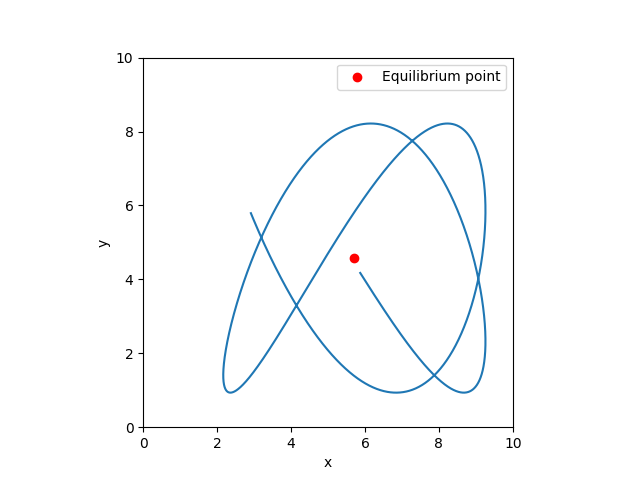
\includegraphics[width=1\linewidth]{example_trajectory_harmonic_oscillator.png}
        \caption{Example trajectory of a body moving due to harmonic oscillator force. The equilibrium position of the harmonic oscillator was also shown. Parameters: $x_{0} = \text{5,87}$, $y_{0} = \text{4,17}$, $V_{0,x} = \text{0,61}$, $V_{0,y} = \text{-0,96}$, $r_{0,x} = \text{5,71}$, $r_{0,y} = \text{4,58}$, $k_{x} = \text{0,03}$, $k_{y} = \text{0,07}$.}
        \label{fig:exmp_traj_harm}
        
        \end{minipage}
    \hfill
        \begin{minipage}{0.49\textwidth}
        
        \centering
        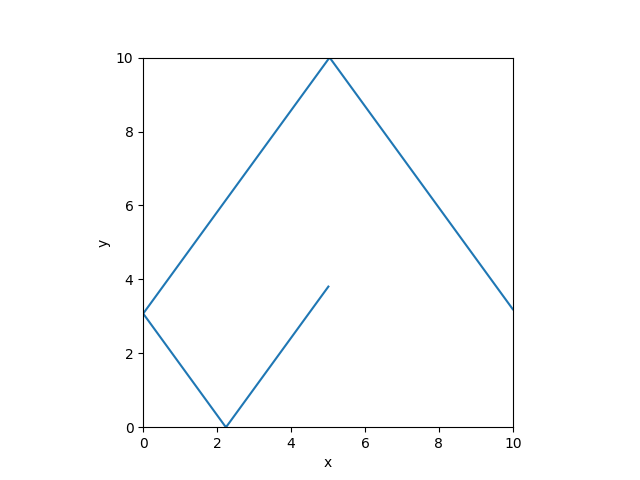
\includegraphics[width=1\linewidth]{example_trajectory_free_body_movement.png}
        \caption{Example trajectory of a body moving freely (no force applied). In this case perfect elastic collisions of the body with walls were implemented. Parameters: $x_{0} = \text{5,01}$, $y_{0} = \text{3,80}$, $V_{0,x} = \text{-0,56}$, $V_{0,y} = \text{-0,77}$.}
        \label{fig:exmp_traj_free}
        
        \end{minipage}  
    \end{figure}
\end{itemize}


For the preliminary results, I used only gravitational simulations. I created 145 simulations with random starting positions, velocities, and directions of the gravity acceleration vector. Each simulation contained about 30 snapshots/frames. Such an example frame is shown in figure~\ref{fig:example_snapshot}.


\begin{figure}[H]

    \centering
    
\includegraphics[width=0.3\textwidth]{example_snapshot.png}
    \caption{An example snapshot of one of the simulations of a body (the red rectangle) moving in a gravity field on the blue background.}
    \label{fig:example_snapshot}

\end{figure}

\subsection{Neural network architecture}

The neural network architecture consists of autoencoder (encoder and decoder) and an evolution operator. The encoder consists of five convolutional ReLU layers (torch.nn.Conv2d and torch.nn.ReLU from PyTorch library) with kernel size 4 and padding 1, four of them with stride 2 followed by one with stride 1. At the end there is a fully connected linear layer (torch.nn.Linear) that gives a latent space vector of dimension 10. The number of channels goes from 3 for the input image to 32, 32, 64, 64 and 256 for the convolutional layers. The encoder can be thought of as a sequence of matrices with progressively smaller number of rows. This means that the dimension of output vector (encoded vector in the latent space) is much smaller than the input vector. The decoder network is a mirror image of the encoder in terms of layer dimensions, with the convolution layers replaced by deconvolution layers (torch.nn.ConvTranspose2d). Analogously, the decoder takes a small encoded vector and maps it to a more dimensional space. The evolution operator has three fully connected 32-neuron layers (torch.nn.Linear) with softplus activation function (torch.nn.Softplus) and a linear 10-neuron output layer. The evolution operator takes two vectors from latent space (the vector from the current and the previous time step) and predicts the latent space vector for the next time step.
A graphical illustration of the architecture is shown in figure~\ref{fig:neural_net_architecture}.

\begin{figure}[H]
    \centering
    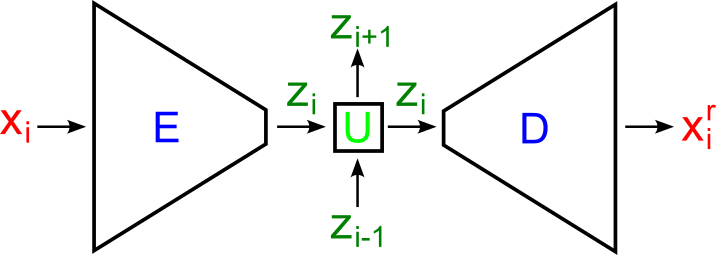
\includegraphics[width=0.5\linewidth]{architecture.png}
    \caption{A draft of a neural network architecture consisting of encoder - E, decoder - D and an evolution operator - U. Encoder E encodes a snapshot from a video (a frame of a video with the moving body) - $x_i$ into a low dimensional latent space vector $z_i$. The evolution operator U takes the latent space vector $z_i$ and the latent space vector from a previous simulation time step - $z_{i-1}$ (we receive it by encoding $x_{i-1}$), and returns the prediction of latent space vector of the following time step $z_{i+1}$. Then, the decoder D decodes the latent space vector $z_i$ and returns the reconstructed snapshot from the video - $x_i^r$. In subsection~\ref{subs:implement_train_loop} an implementation of the training loop of the network was presented. The symbols used on the figure correspond to the variables used in the code, in the following way: $x_i=\text{x\_i}$, $z_i=\text{z\_i}$, $z_{i-1}=\text{z\_prev}$, $z_{i+1}=\text{z\_next\_pred}$, $x_i^r=\text{reconstructed}$ (in the code these variables appear for example in the line 67).}
    \label{fig:neural_net_architecture}
\end{figure}

\subsection{Loss function}
\label{subs:loss_function}

The learning process of a neural network model is governed by the loss function $\mathcal{L}$, which tells us how well a given model already learnt. The gradients of $\mathcal{L}$ with respect to the "matrix entries" called weights $\omega_i$ will serve as learning "steps" such that:

\begin{equation*}
    \omega_i\rightarrow\omega_i +\alpha^*\frac{\partial \mathcal{L}}{\partial \omega_i},
\end{equation*}

\nid where $\alpha^*$ is a hyperparameter of the learning process called learning rate.

The loss function~\cite{Udrescu2021} was implemented as follows:

\begin{equation}
\label{eq:loss_function}
    \mathcal{L} = \mathcal{L}^{recon} + \alpha\mathcal{L}^{pred} + \beta\mathcal{L}^{nl} + \gamma\mathcal{L}^{acc}. 
\end{equation}

\nid These four terms are averages over all time steps \txt{i} of the following functions:

\begin{flushleft}
    \begin{align*}
        \mathcal{L}^{recon}_i & = \frac{|x_i-D(E(x_i))|}{|x_i|},\\
        \mathcal{L}^{pred}_i & = \frac{|z_{i+1} - U(z_i, z_{i-1})|}{|z_i - z_{i-1}|},\\
        \mathcal{L}^{nl}_i & = \frac{1}{4000}|z_i - z_{i-1}|\cdot||\nabla\boldsymbol{J}(\boldsymbol{w}_i)||_1,\\ 
        \mathcal{L}^{acc}_i & = \frac{1}{10}||U(\boldsymbol{w}_i) - \boldsymbol{M}\boldsymbol{w}_i||_1,
    \end{align*}
\end{flushleft}

\nid where $\alpha$, $\beta$, $\gamma$ are tunable hyperparameters, $\mathbf{w}_i = \begin{pmatrix} z_{i-1} \\ z_{i} \end{pmatrix}$, $\boldsymbol{J}$ is the Jacobian of an evolution operator U, $\boldsymbol{M} = \begin{pmatrix} -\boldsymbol{I} & 2\boldsymbol{I} \end{pmatrix}$ and $\boldsymbol{I}$ is the 10x10 identity matrix. 

$\mathcal{L}^{recon}$ is the reconstruction error - it simply tells how good the encoder-decoder architecture preserves the input image, which we want to as good as possible. $\mathcal{L}^{pred}$ is the prediction error which tells how well the evolution operator \txt{U} predicts the next latent space vector from two previous ones, which we also want to be as good as possible, so that the dynamics of the moving body is described well. $\mathcal{L}^{nl}$ is a measure of the nonlinearity of the mapping \txt{U}, since its Jacobian $\boldsymbol{J}$ will be constant if the mapping is linear, i.e. the dynamics of the body is described by coupled linear differential equations, which encompass behaviour such as motion in magnetic fields, harmonic oscillator potential and gravity. $\mathcal{L}^{acc}$ is along with $\mathcal{L}^{nl}$ yet another measure of the nonlinearity of the mapping U and is a measure of the predicted acceleration. There is no acceleration if the mapping is $U(\boldsymbol{w}) = \boldsymbol{M}\boldsymbol{w}$.

To obtain the preliminary results, that I show in the paper, I used only the first part of the loss function - $\mathcal{L}^{recon}$.

\subsection{Implementation of the training loop}
\label{subs:implement_train_loop}

In this subsection I present the code implementation of the training loop. 

\begin{lstlisting}
# Third party imports:
import torch
from tqdm import tqdm

# Self written library imports:
import datasets
import autoencoder
import visualization
import evaluator


def train_autoencoder(model, train_loader, val_loader, epochs=10, initial_lr=0.001, lr_decay_step=10, lr_decay_factor=0.9, save_model=False, device='cuda' if torch.cuda.is_available() else 'cpu'):

    # Move model to GPU if available:
    model.to(device)
    
    # Define optimizer:
    optimizer = torch.optim.Adam(model.parameters(), lr=initial_lr)

    # Define learning rate scheduler:
    scheduler = torch.optim.lr_scheduler.StepLR(optimizer, step_size=lr_decay_step, gamma=lr_decay_factor)

    # Store loss values:
    history = {"loss": [], "val_loss": []}

    # Instantiate the loss function:
    recon_loss_fn = evaluator.ReconstructionError()

    for epoch in range(epochs):
        total_loss = 0.0
        val_loss = 0.0
        # Code for showing progress bar of each training epoch:
        progress_bar = tqdm(train_loader, desc=f"Epoch {epoch + 1}/{epochs}")

        for batch in progress_bar:
            batch = batch.to(device)

            x_prev, x_i, x_next = batch[:, 0], batch[:, 1], batch[:, 2]

            optimizer.zero_grad()
            reconstructed, z_i, z_next_pred = model(x_i, z_prev=model.encoder(x_prev))

            # Calculating loss:
            loss = recon_loss_fn(x_i, reconstructed)

            # Loss backward propagation:
            loss.backward()
            optimizer.step()

            total_loss += loss.item()

            # Update tqdm progress bar with loss:
            progress_bar.set_postfix(loss=f"{total_loss:.4f}")

        history["loss"].append(total_loss / len(train_loader))

        # Step the scheduler after every epoch
        scheduler.step()

        # Validation loop:
        model.eval()  # Set model to evaluation mode (no change of weights)
        with torch.no_grad():
            for batch in val_loader:
                batch = batch.to(device)
                x_prev, x_i, x_next = batch[:, 0], batch[:, 1], batch[:, 2]

                reconstructed, z_i, z_next_pred = model(x_i, z_prev=model.encoder(x_prev))

                # Calculating loss:
                loss = recon_loss_fn(x_i, reconstructed)
                val_loss = loss.item()

        model.train()  # Set model back to training mode
        history["val_loss"].append(val_loss / len(val_loader))

        # Print current loss and learning rate
        current_lr = scheduler.get_last_lr()[0]
        print(f"Epoch {epoch + 1} - Avg. Train Loss: {history['loss'][-1]:.4f}, "
              f"Avg. Val Loss: {history['val_loss'][-1]:.4f}, LR: {current_lr:.6f}")

    print("Training complete!")

    if save_model:
        torch.save(model.state_dict(),
        fr'saved_models/trained_on_{epochs}_simul_lr_params_'
        fr'{initial_lr}_{lr_decay_step}_{lr_decay_factor}_recon_loss_'
        fr'only_latent_dim_{model.latent_dim}.pth')
        print("Model saved!")

    return history


if __name__ == '__main__':
    # Instantiate the model:
    model = autoencoder.AutoencoderWithEvolution(latent_dim=10)

    # Load dataset using DataLoader:
    dataset = datasets.LoadedDataset()

    # Split dataset into training and validation sets:
    # The dataset conatains triplets of consecutive images from the simulations of a body moving in a gravity field
    train_size = int(0.8 * len(dataset))  # 80% for training
    val_size = len(dataset) - train_size  # 20% for validation
    train_dataset, val_dataset = torch.utils.data.random_split(dataset, [train_size, val_size])

    # Create DataLoaders:
    train_loader = torch.utils.data.DataLoader(train_dataset, batch_size=128, shuffle=True)
    val_loader = torch.utils.data.DataLoader(val_dataset, batch_size=128, shuffle=False)

    # Train the model:
    history = train_autoencoder(model, train_loader, val_loader, epochs=400, save_model=True, initial_lr=1.e-3,
                                lr_decay_step=25)

    # Plot the loss history:
    visualization.plot_train_history(history)
\end{lstlisting}

\section{Preliminary results}

In the figure~\ref{graph:loss_function_vs_epoch_number} I show the change of loss function (in this case I used only reconstruction part of the total loss function~\ref{eq:loss_function}) with respect to epoch of the training. Each epoch of the training corresponds to training performed on gravity simulation snapshots (about 4000 images in total). During the first attempts, I struggled with the model not learning to reconstruct the red rectangle in the image but only the blue background. Allowing the model to train for a longer number of epochs allowed it to find a way to get out of the "background" minimum. The comparison between an original image and the reconstructed one is shown in figure~\ref{fig:original_reconstructed_image}. 

I also created an image of a reconstructed trajectory for one of the gravity simulations (about 30 images), which is shown in the figure~\ref{fig:original_reconstructed_trajectory}. The latent space dimension for the model I used here is 10. I reduced the dimension to 2 using principal component analysis. As one could predict the reconstructed trajectory and the original one are not similar as the loss function used lacked the terms that are responsible for learning the model proper latent space representation.

\begin{figure}[H]
    \centering
    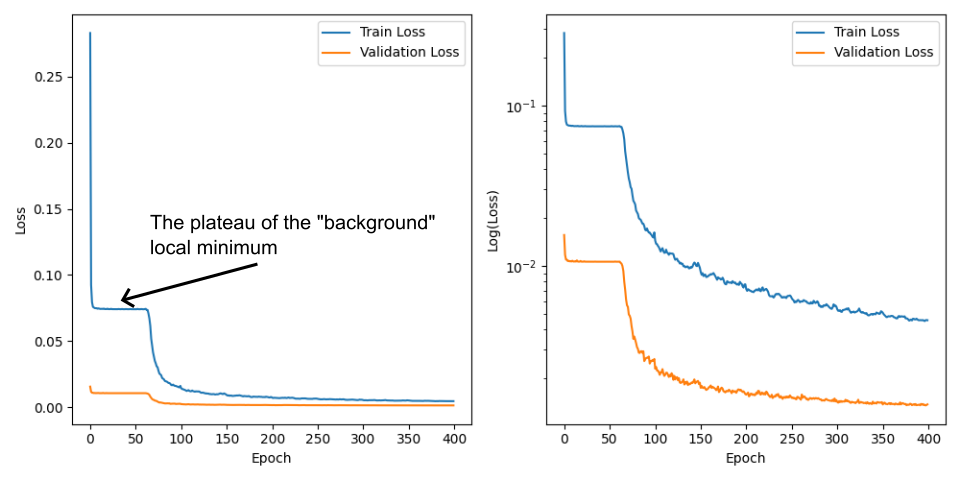
\includegraphics[width=1\linewidth]{loss_history.png}
    \caption{Value of reconstruction error $\mathcal{L}^{recon}$ with respect to epoch of the model training (linear scale on the left and logarithmic scale one the right). Each epoch corresponds to training performed on gravity simulation snapshots (about 4000 images in total). The arrow shows a part of the training, in which the model falls into a local minimum that makes it reconstruct the blue background only, i.e. without the red rectangle.}
    \label{graph:loss_function_vs_epoch_number}
\end{figure}

\begin{figure}[H]
    \centering

    \begin{minipage}{0.49\textwidth}
    
    \centering
    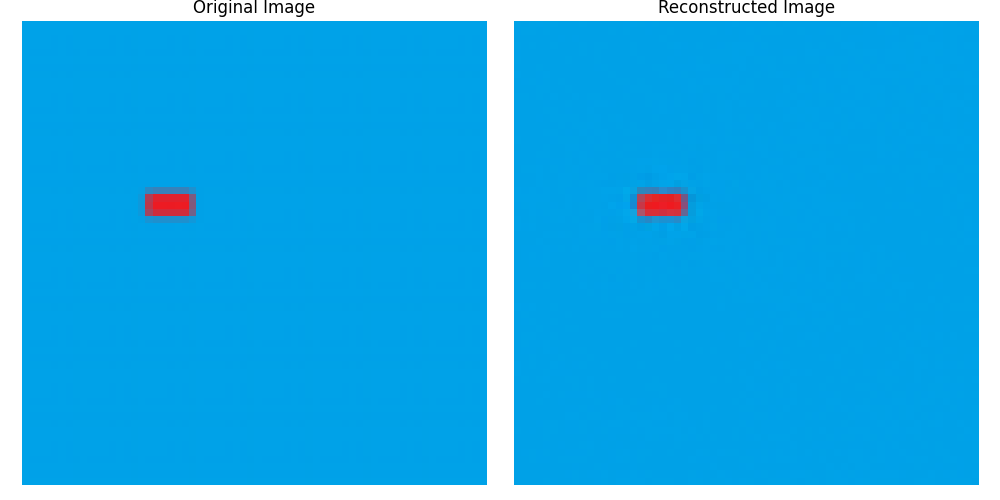
\includegraphics[width=1\textwidth]{reconstruction_example.png}
    \caption{The comparison between original snapshot of a simulation (the photo is blurred as the images entering encoder are deliberately downsampled) on the left and the reconstructed image on the right.}
    \label{fig:original_reconstructed_image}
    
    \end{minipage}
    \hfill
    \begin{minipage}{0.49\textwidth}
    
    \centering
    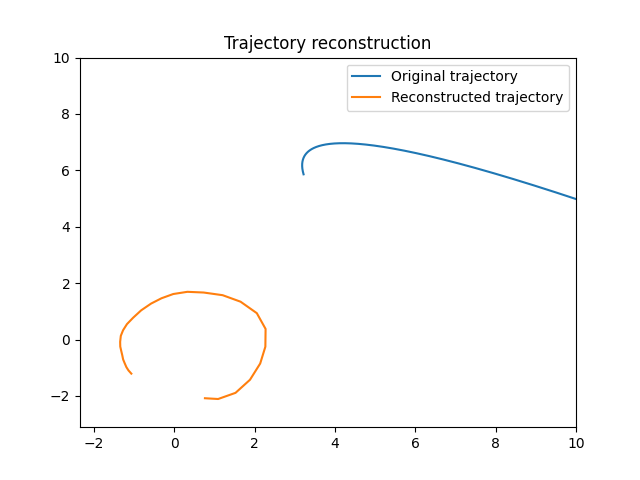
\includegraphics[width=1\textwidth]{trajectory_reconstruction.png}
    \caption{The comparison between the original trajectory of a body on the left with the reconstructed trajectory on the left.}
    \label{fig:original_reconstructed_trajectory}

    \end{minipage}    
    
\end{figure}


\section{Summary and future work}

In the paper I presented the preliminary results of my attempt to reproduce the results of the article~\cite{Udrescu2021}. For now, I did not manage to obtain a correctly working algorithm that reconstructs the trajectory of a moving object from a video as I only used a part of the loss function (i.e. reconstruction error).

In the future work, I will concentrate on extending the loss function and try to obtain the desired results. The work that is still ahead is implementing a comprehensive evaluator that would assess the quality of latent space trajectory representations and extending the training of the model on other types of motion like movement in magnetic field, harmonic oscillator. In the end it would be interesting to see, if the neural network architecture would be able to detect the trajectories of bodies from real footages. 

Personally, it was my first approach to a serious application of machine learning, especially neural networks. The project allowed me to understand the process of preparing data for training, training and debugging a neural network model using PyTorch library.

The machine learning approach is also important in much more prestigious subjects of physics than Newtonian mechanics. Computational physics or results analysis of experiments performed at LHC~\cite{ARPAIA2021} are examples of that.  

\printbibliography

\end{document}
